\documentclass[]{article}
\usepackage{ctex} %中文支持
%opening
\title{图表释义}
\author{李蕴哲}

\begin{document}

\maketitle

%\begin{abstract}

%\end{abstract}

\section{设定}

标签设定为:

\begin{itemize}
	\item 2为初中生组
	\item 3为高中生组
	\item 4为大学生组
\end{itemize}

中英文为同样的文本,作者为中文母语,统计量为过去式的个数。

中文分词及词性判别采用jieba分词工具\footnote{结巴分词工具可见:https://github.com/fxsjy/jieba},判断标准为是否出现了“了”。英文分词及词性判别采用Natural Language Toolkit (nltk) 分词工具\footnote{nltk分词工具可见:https://www.nltk.org/},判断标准为是否存在过去式。

\section{箱线图}

箱线图,显示一组数据分散情况的统计图。形状如箱子。主要用于反映原始数据分布的特征,关键的5个黑线是最大值、最小值、中位数和两个四分位数。

中英文的两个箱线图如图\ref{fig:xxc}和图\ref{fig:xxe}所示。

\begin{figure}
	\centering
	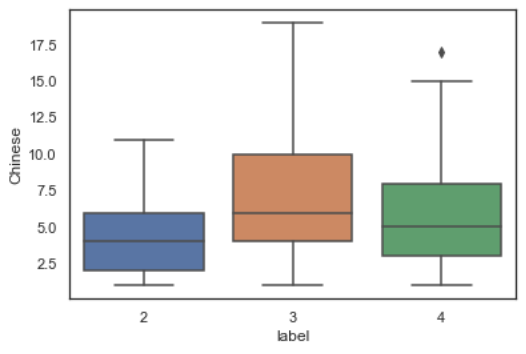
\includegraphics[width=0.7\linewidth]{fig/xxc}
	\caption{中文过去式数量统计箱线图}
	\label{fig:xxc}
\end{figure}

\begin{figure}
	\centering
	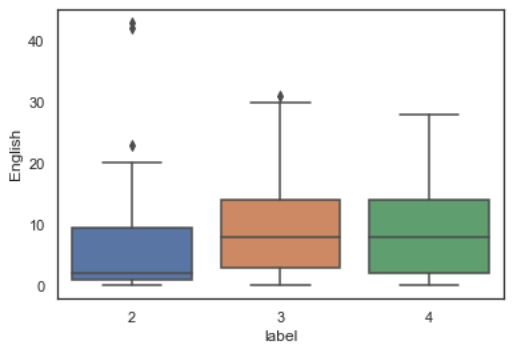
\includegraphics[width=0.7\linewidth]{fig/xxe}
	\caption{英文过去式数量统计箱线图}
	\label{fig:xxe}
\end{figure}

以图\ref{fig:xxc}为例,标签为2的箱线图最高的黑线为11左右,这是初中生组中文文本中存在的过去式数量的最大值,第二根黑线为7左右,这是第一个四分位数\footnote{第一个四分位数为第75\%大的数}。第三根黑线为中位数,约为4。第四根黑线为第二个四分位数\footnote{第二个四分位数为第25\%大的数},约为2。第五根黑线即为最低的数量,约为1,为最小值。其他箱线以此类推。

可以看出,不管是初中生、高中生还是大学生,就群体而言,两种语言过去式的数量总是相似的。但是,大学生两种语言过去式的数量的吻合程度更好。初中生倾向于少用英文过去式,或许是因为语法掌握不当;高中生过去式用得很多,或许是因为语言较为生硬。

\section{散点图}

散点图是指在回归分析中,数据点在直角坐标系平面上的分布图,散点图表示因变量随自变量而变化的大致趋势。

不同类别的学习者中英文过去式数量的散点图如图\ref{fig:sdtt}所示。

\begin{figure}
	\centering
	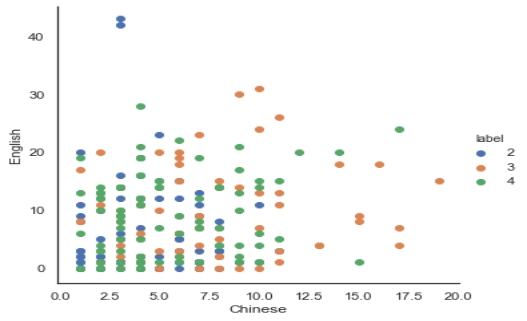
\includegraphics[width=0.7\linewidth]{fig/sdtt}
	\caption{中英文过去式数量散点图}
	\label{fig:sdtt}
\end{figure}

图\ref{fig:sdtt}中,横坐标为同一学习者在中文文本中的过去式数量,纵坐标是在英文文本中的过去式数量。不同的类别使用不同颜色的点加以区分。例如,如果一个点的横坐标为5,纵坐标为12,那么意味着这位语言学习者的同样的文本中中文过去式数量为5,英文过去式数量为12。

从图中可以看出,过去式的使用较为杂乱无章,几乎没有规律。因此将图\ref{fig:sdtt}拆开,拆成图\ref{fig:sdt2}、图\ref{fig:sdt3}和图\ref{fig:sdt4}。

\begin{figure}
	\centering
	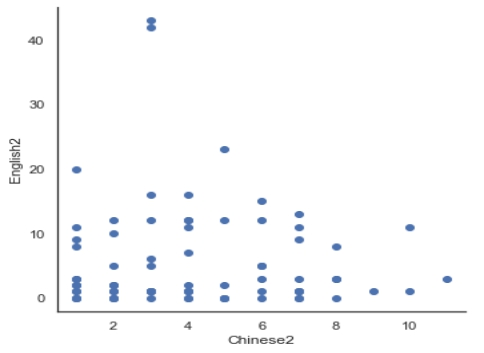
\includegraphics[width=0.7\linewidth]{fig/sdt2}
	\caption{初中生中英文过去式数量散点图}
	\label{fig:sdt2}
\end{figure}

\begin{figure}
	\centering
	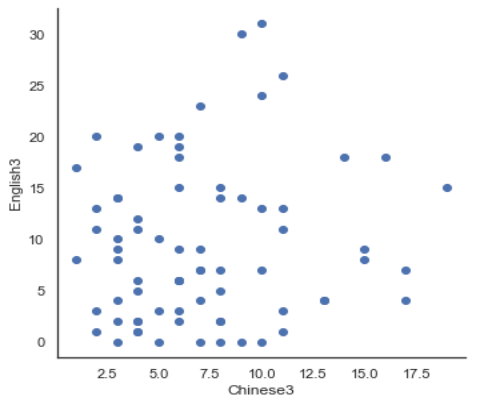
\includegraphics[width=0.7\linewidth]{fig/sdt3}
	\caption{高中生中英文过去式数量散点图}
	\label{fig:sdt3}
\end{figure}

\begin{figure}
	\centering
	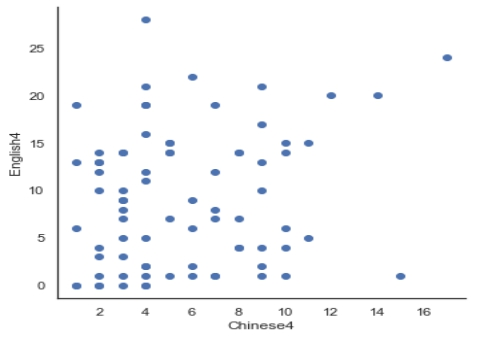
\includegraphics[width=0.7\linewidth]{fig/sdt4}
	\caption{大学生中英文过去式数量散点图}
	\label{fig:sdt4}
\end{figure}

这三个图看似凌乱,但是也可以看出因语言学习者学习阶段的不同而呈现的一些规律:

\begin{enumerate}
	\item 总体上,同一学习者中英文文本中过去式数量并没有特别大的关联,且中文的过去式数量明显小于英文文本,这或许意味着过去式的使用普遍存在着不规范的问题。
	\item 从初中生到高中生到大学生,过去式的数量之间渐渐的体现出了一定的正相关性。初中生的文本中很多数据点看不出关联,高中生的文本中渐渐地已经能感受到随着中文文本的过去式的增加英文的过去式数量也在增多,而大学生的文本中这样的趋势已经很明显了。这体现了随着学习时间的增加,过去式使用的规范。如果可以调研更高层次的学习者,比如博士群体或者英专学生,或许这样的关联会更加明显。
\end{enumerate}

\section{散点图线性拟合}

本节对散点图进行一些拟合分析。

\subsection{最小二乘法}

LinearRegression\cite{sklearn} 拟合一个带有系数 $w = (w_1, ..., w_p) $ 的线性模型,使得数据集实际观测数据和预测数据(估计值)之间的残差平方和最小。其数学表达式为:

\begin{equation}
\min_w\|Xw-y\|_2^2
\end{equation}

\subsection{拟合结果}

三个图的拟合结果\footnote{使用sklearn进行拟合,sklearn可见:https://scikit-learn.org/}如图\ref{fig:nh2}、图\ref{fig:nh3}和图\ref{fig:nh4}所示。

\begin{figure}
	\centering
	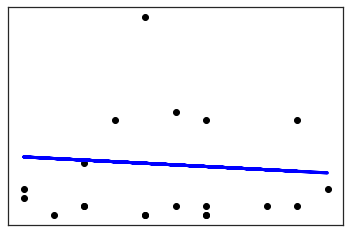
\includegraphics[width=0.7\linewidth]{fig/nh2}
	\caption{初中生散点图拟合结果}
	\label{fig:nh2}
\end{figure}

\begin{figure}
	\centering
	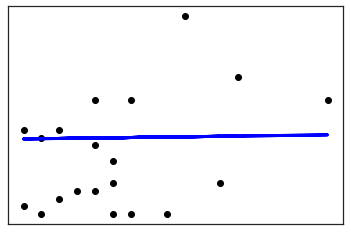
\includegraphics[width=0.7\linewidth]{fig/nh3}
	\caption{高中生拟合结果}
	\label{fig:nh3}
\end{figure}

\begin{figure}
	\centering
	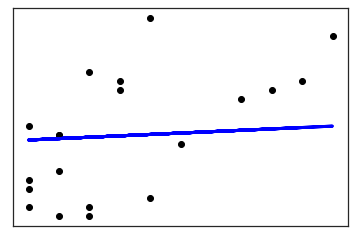
\includegraphics[width=0.7\linewidth]{fig/nh4}
	\caption{大学生拟合结果}
	\label{fig:nh4}
\end{figure}

图中的点为测试集\footnote{在机器学习中,往往会以一定的原则划分训练集和测试集,训练集用于学习特征,测试集用于检测学习的效果。这里使用的方法为随机划分。}的样本,线为拟合的结果,也就是说,如果数据没有误差的话,应当分布在这条线上。拟合的系数即为这条线的斜率\footnote{斜率即为直线的倾斜程度,可参考:https://en.wikipedia.org/wiki/Slope}。

初中生组的拟合的系数为-0.18624161,测试集均方误差\footnote{均方误差为一种衡量结果好坏的指标,可参考:https://en.wikipedia.org/wiki/Mean\_squared\_error}为38.50;高中生组的拟合系数为0.03147746,测试集均方误差为55.48;大学生组的拟合系数为0.15457223,测试集均方误差为41.15。

\subsection{结果分析}

直觉上,同一个文本的过去式数量,不管语言,应该是正相关的,也就是说,线性拟合的系数应该是正的,并且为某一确切的正值(直觉上这一值应当是大于1的)。与此同时,回归的误差应当比较小,说明特征的一致性。

初中生、高中生和大学生的拟合结果正反应了这一特征。初中生的数据几乎无法拟合,拟合出来的结果是负相关,完全是错误的;高中生的数据拟合出来的系数比较小,而均方误差比较大;大学生的系数较大,均方误差相对于高中生较小。

\subsection{局限性}

数据效果比较差,这一特征体现并不明显。同时,数据量过小,这样的结果存在过拟合\footnote{过拟合即学到的特征是这一数据集特有的特征,而非我们想要研究的通用特征,可参考:https://en.wikipedia.org/wiki/Overfitting}的可能。

\begin{thebibliography}{99}  
	\bibitem{sklearn}“1.1. 广义线性模型 · sklearn 中文文档.” [Online]. Available: https://sklearn.apachecn.org/docs/0.21.3/2.html. [Accessed: 14-Mar-2020].
	
\end{thebibliography}

\end{document}
